\documentclass[1p]{elsarticle_modified}
%\bibliographystyle{elsarticle-num}

%\usepackage[colorlinks]{hyperref}
%\usepackage{abbrmath_seonhwa} %\Abb, \Ascr, \Acal ,\Abf, \Afrak
\usepackage{amsfonts}
\usepackage{amssymb}
\usepackage{amsmath}
\usepackage{amsthm}
\usepackage{scalefnt}
\usepackage{amsbsy}
\usepackage{kotex}
\usepackage{caption}
\usepackage{subfig}
\usepackage{color}
\usepackage{graphicx}
\usepackage{xcolor} %% white, black, red, green, blue, cyan, magenta, yellow
\usepackage{float}
\usepackage{setspace}
\usepackage{hyperref}

\usepackage{tikz}
\usetikzlibrary{arrows}

\usepackage{multirow}
\usepackage{array} % fixed length table
\usepackage{hhline}

%%%%%%%%%%%%%%%%%%%%%
\makeatletter
\renewcommand*\env@matrix[1][\arraystretch]{%
	\edef\arraystretch{#1}%
	\hskip -\arraycolsep
	\let\@ifnextchar\new@ifnextchar
	\array{*\c@MaxMatrixCols c}}
\makeatother %https://tex.stackexchange.com/questions/14071/how-can-i-increase-the-line-spacing-in-a-matrix
%%%%%%%%%%%%%%%

\usepackage[normalem]{ulem}

\newcommand{\msout}[1]{\ifmmode\text{\sout{\ensuremath{#1}}}\else\sout{#1}\fi}
%SOURCE: \msout is \stkout macro in https://tex.stackexchange.com/questions/20609/strikeout-in-math-mode

\newcommand{\cancel}[1]{
	\ifmmode
	{\color{red}\msout{#1}}
	\else
	{\color{red}\sout{#1}}
	\fi
}

\newcommand{\add}[1]{
	{\color{blue}\uwave{#1}}
}

\newcommand{\replace}[2]{
	\ifmmode
	{\color{red}\msout{#1}}{\color{blue}\uwave{#2}}
	\else
	{\color{red}\sout{#1}}{\color{blue}\uwave{#2}}
	\fi
}

\newcommand{\Sol}{\mathcal{S}} %segment
\newcommand{\D}{D} %diagram
\newcommand{\A}{\mathcal{A}} %arc


%%%%%%%%%%%%%%%%%%%%%%%%%%%%%5 test

\def\sl{\operatorname{\textup{SL}}(2,\Cbb)}
\def\psl{\operatorname{\textup{PSL}}(2,\Cbb)}
\def\quan{\mkern 1mu \triangleright \mkern 1mu}

\theoremstyle{definition}
\newtheorem{thm}{Theorem}[section]
\newtheorem{prop}[thm]{Proposition}
\newtheorem{lem}[thm]{Lemma}
\newtheorem{ques}[thm]{Question}
\newtheorem{cor}[thm]{Corollary}
\newtheorem{defn}[thm]{Definition}
\newtheorem{exam}[thm]{Example}
\newtheorem{rmk}[thm]{Remark}
\newtheorem{alg}[thm]{Algorithm}

\newcommand{\I}{\sqrt{-1}}
\begin{document}

%\begin{frontmatter}
%
%\title{Boundary parabolic representations of knots up to 8 crossings}
%
%%% Group authors per affiliation:
%\author{Yunhi Cho} 
%\address{Department of Mathematics, University of Seoul, Seoul, Korea}
%\ead{yhcho@uos.ac.kr}
%
%
%\author{Seonhwa Kim} %\fnref{s_kim}}
%\address{Center for Geometry and Physics, Institute for Basic Science, Pohang, 37673, Korea}
%\ead{ryeona17@ibs.re.kr}
%
%\author{Hyuk Kim}
%\address{Department of Mathematical Sciences, Seoul National University, Seoul 08826, Korea}
%\ead{hyukkim@snu.ac.kr}
%
%\author{Seokbeom Yoon}
%\address{Department of Mathematical Sciences, Seoul National University, Seoul, 08826,  Korea}
%\ead{sbyoon15@snu.ac.kr}
%
%\begin{abstract}
%We find all boundary parabolic representation of knots up to 8 crossings.
%
%\end{abstract}
%\begin{keyword}
%    \MSC[2010] 57M25 
%\end{keyword}
%
%\end{frontmatter}

%\linenumbers
%\tableofcontents
%
\newcommand\colored[1]{\textcolor{white}{\rule[-0.35ex]{0.8em}{1.4ex}}\kern-0.8em\color{red} #1}%
%\newcommand\colored[1]{\textcolor{white}{ #1}\kern-2.17ex	\textcolor{white}{ #1}\kern-1.81ex	\textcolor{white}{ #1}\kern-2.15ex\color{red}#1	}

{\Large $\underline{12n_{0039}~(K12n_{0039})}$}

\setlength{\tabcolsep}{10pt}
\renewcommand{\arraystretch}{1.6}
\vspace{1cm}\begin{tabular}{m{100pt}>{\centering\arraybackslash}m{274pt}}
\multirow{5}{120pt}{
	\centering
	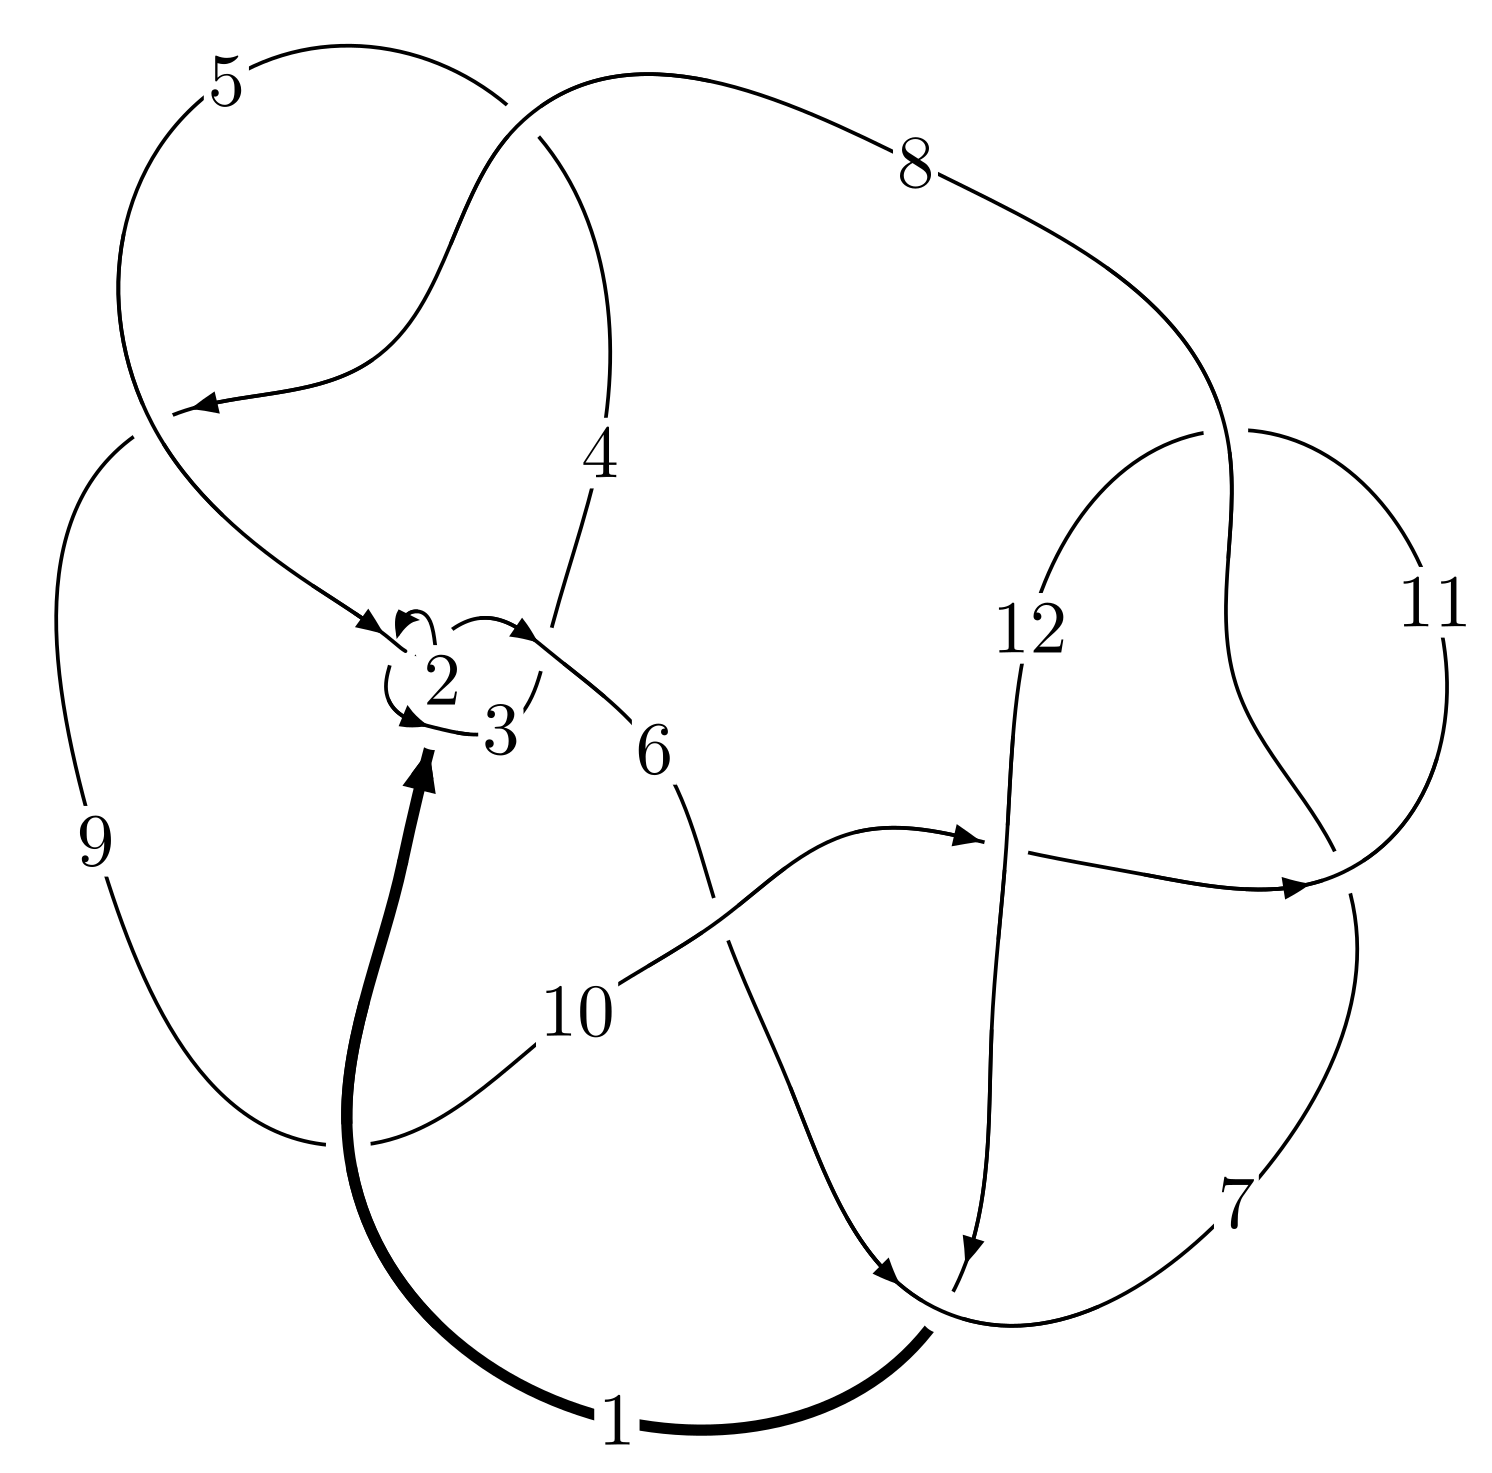
\includegraphics[width=112pt]{../../../GIT/diagram.site/Diagrams/png/2128_12n_0039.png}\\
\ \ \ A knot diagram\footnotemark}&
\allowdisplaybreaks
\textbf{Linearized knot diagam} \\
\cline{2-2}
 &
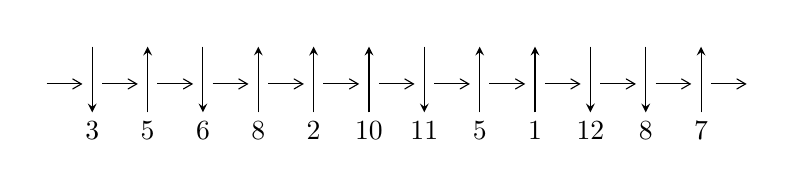
\begin{tikzpicture}[x=20pt, y=17pt]
	% nodes
	\node (C0) at (0, 0) {};
	\node (C1) at (1, 0) {};
	\node (C1U) at (1, +1) {};
	\node (C1D) at (1, -1) {3};

	\node (C2) at (2, 0) {};
	\node (C2U) at (2, +1) {};
	\node (C2D) at (2, -1) {5};

	\node (C3) at (3, 0) {};
	\node (C3U) at (3, +1) {};
	\node (C3D) at (3, -1) {6};

	\node (C4) at (4, 0) {};
	\node (C4U) at (4, +1) {};
	\node (C4D) at (4, -1) {8};

	\node (C5) at (5, 0) {};
	\node (C5U) at (5, +1) {};
	\node (C5D) at (5, -1) {2};

	\node (C6) at (6, 0) {};
	\node (C6U) at (6, +1) {};
	\node (C6D) at (6, -1) {10};

	\node (C7) at (7, 0) {};
	\node (C7U) at (7, +1) {};
	\node (C7D) at (7, -1) {11};

	\node (C8) at (8, 0) {};
	\node (C8U) at (8, +1) {};
	\node (C8D) at (8, -1) {5};

	\node (C9) at (9, 0) {};
	\node (C9U) at (9, +1) {};
	\node (C9D) at (9, -1) {1};

	\node (C10) at (10, 0) {};
	\node (C10U) at (10, +1) {};
	\node (C10D) at (10, -1) {12};

	\node (C11) at (11, 0) {};
	\node (C11U) at (11, +1) {};
	\node (C11D) at (11, -1) {8};

	\node (C12) at (12, 0) {};
	\node (C12U) at (12, +1) {};
	\node (C12D) at (12, -1) {7};
	\node (C13) at (13, 0) {};

	% arrows
	\draw[->,>={angle 60}]
	(C0) edge (C1) (C1) edge (C2) (C2) edge (C3) (C3) edge (C4) (C4) edge (C5) (C5) edge (C6) (C6) edge (C7) (C7) edge (C8) (C8) edge (C9) (C9) edge (C10) (C10) edge (C11) (C11) edge (C12) (C12) edge (C13) ;	\draw[->,>=stealth]
	(C1U) edge (C1D) (C2D) edge (C2U) (C3U) edge (C3D) (C4D) edge (C4U) (C5D) edge (C5U) (C6D) edge (C6U) (C7U) edge (C7D) (C8D) edge (C8U) (C9D) edge (C9U) (C10U) edge (C10D) (C11U) edge (C11D) (C12D) edge (C12U) ;
	\end{tikzpicture} \\
\hhline{~~} \\& 
\textbf{Solving Sequence} \\ \cline{2-2} 
 &
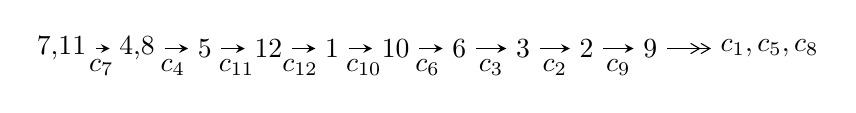
\begin{tikzpicture}[x=23pt, y=7pt]
	% node
	\node (A0) at (-1/8, 0) {7,11};
	\node (A1) at (17/16, 0) {4,8};
	\node (A2) at (17/8, 0) {5};
	\node (A3) at (25/8, 0) {12};
	\node (A4) at (33/8, 0) {1};
	\node (A5) at (41/8, 0) {10};
	\node (A6) at (49/8, 0) {6};
	\node (A7) at (57/8, 0) {3};
	\node (A8) at (65/8, 0) {2};
	\node (A9) at (73/8, 0) {9};
	\node (C1) at (1/2, -1) {$c_{7}$};
	\node (C2) at (13/8, -1) {$c_{4}$};
	\node (C3) at (21/8, -1) {$c_{11}$};
	\node (C4) at (29/8, -1) {$c_{12}$};
	\node (C5) at (37/8, -1) {$c_{10}$};
	\node (C6) at (45/8, -1) {$c_{6}$};
	\node (C7) at (53/8, -1) {$c_{3}$};
	\node (C8) at (61/8, -1) {$c_{2}$};
	\node (C9) at (69/8, -1) {$c_{9}$};
	\node (A10) at (11, 0) {$c_{1},c_{5},c_{8}$};

	% edge
	\draw[->,>=stealth]	
	(A0) edge (A1) (A1) edge (A2) (A2) edge (A3) (A3) edge (A4) (A4) edge (A5) (A5) edge (A6) (A6) edge (A7) (A7) edge (A8) (A8) edge (A9) ;
	\draw[->>,>={angle 60}]	
	(A9) edge (A10);
\end{tikzpicture} \\ 

\end{tabular} \\

\footnotetext{
The image of knot diagram is generated by the software ``\textbf{Draw programme}" developed by Andrew Bartholomew(\url{http://www.layer8.co.uk/maths/draw/index.htm\#Running-draw}), where we modified some parts for our purpose(\url{https://github.com/CATsTAILs/LinksPainter}).
}\phantom \\ \newline 
\centering \textbf{Ideals for irreducible components\footnotemark of $X_{\text{par}}$} 
 
\begin{align*}
I^u_{1}&=\langle 
- u^{57}- u^{56}+\cdots+2 b-4,\;13 u^{57}-29 u^{56}+\cdots+2 a-9,\;u^{58}-3 u^{57}+\cdots-3 u+1\rangle \\
I^u_{2}&=\langle 
- u^2 a+b,\;- u^4 a- u^3 a+u^2 a- u^3+a^2+a u- u^2+1,\;u^6+u^5- u^4-2 u^3+u+1\rangle \\
\\
\end{align*}
\raggedright * 2 irreducible components of $\dim_{\mathbb{C}}=0$, with total 70 representations.\\
\footnotetext{All coefficients of polynomials are rational numbers. But the coefficients are sometimes approximated in decimal forms when there is not enough margin.}
\newpage
\renewcommand{\arraystretch}{1}
\centering \section*{I. $I^u_{1}= \langle - u^{57}- u^{56}+\cdots+2 b-4,\;13 u^{57}-29 u^{56}+\cdots+2 a-9,\;u^{58}-3 u^{57}+\cdots-3 u+1 \rangle$}
\flushleft \textbf{(i) Arc colorings}\\
\begin{tabular}{m{7pt} m{180pt} m{7pt} m{180pt} }
\flushright $a_{7}=$&$\begin{pmatrix}1\\0\end{pmatrix}$ \\
\flushright $a_{11}=$&$\begin{pmatrix}0\\u\end{pmatrix}$ \\
\flushright $a_{4}=$&$\begin{pmatrix}-\frac{13}{2} u^{57}+\frac{29}{2} u^{56}+\cdots-\frac{33}{2} u+\frac{9}{2}\\\frac{1}{2} u^{57}+\frac{1}{2} u^{56}+\cdots-\frac{1}{2} u+2\end{pmatrix}$ \\
\flushright $a_{8}=$&$\begin{pmatrix}1\\u^2\end{pmatrix}$ \\
\flushright $a_{5}=$&$\begin{pmatrix}-\frac{7}{2} u^{57}+\frac{15}{2} u^{56}+\cdots-\frac{17}{2} u+\frac{3}{2}\\\frac{3}{2} u^{57}-\frac{5}{2} u^{56}+\cdots-3 u^2+\frac{5}{2} u\end{pmatrix}$ \\
\flushright $a_{12}=$&$\begin{pmatrix}- u\\- u^3+u\end{pmatrix}$ \\
\flushright $a_{1}=$&$\begin{pmatrix}- u^3\\- u^3+u\end{pmatrix}$ \\
\flushright $a_{10}=$&$\begin{pmatrix}u^3\\u^5- u^3+u\end{pmatrix}$ \\
\flushright $a_{6}=$&$\begin{pmatrix}u^8- u^6+u^4+1\\u^{10}-2 u^8+3 u^6-2 u^4+u^2\end{pmatrix}$ \\
\flushright $a_{3}=$&$\begin{pmatrix}-5 u^{57}+11 u^{56}+\cdots-\frac{23}{2} u+\frac{7}{2}\\u^{57}- u^{56}+\cdots+\frac{3}{2} u+1\end{pmatrix}$ \\
\flushright $a_{2}=$&$\begin{pmatrix}- u^{57}+2 u^{56}+\cdots-\frac{3}{2} u+\frac{3}{2}\\\frac{1}{2} u^{54}-\frac{1}{2} u^{53}+\cdots+\frac{1}{2} u^2+\frac{1}{2} u\end{pmatrix}$ \\
\flushright $a_{9}=$&$\begin{pmatrix}- u^{11}+2 u^9-2 u^7+u^3\\- u^{11}+3 u^9-4 u^7+3 u^5- u^3+u\end{pmatrix}$\\&\end{tabular}
\flushleft \textbf{(ii) Obstruction class $= -1$}\\~\\
\flushleft \textbf{(iii) Cusp Shapes $= 12 u^{57}-\frac{51}{2} u^{56}+\cdots+\frac{53}{2} u-6$}\\~\\
\newpage\renewcommand{\arraystretch}{1}
\flushleft \textbf{(iv) u-Polynomials at the component}\newline \\
\begin{tabular}{m{50pt}|m{274pt}}
Crossings & \hspace{64pt}u-Polynomials at each crossing \\
\hline $$\begin{aligned}c_{1}\end{aligned}$$&$\begin{aligned}
&u^{58}+35 u^{57}+\cdots+9 u+1
\end{aligned}$\\
\hline $$\begin{aligned}c_{2},c_{5}\end{aligned}$$&$\begin{aligned}
&u^{58}+7 u^{57}+\cdots+5 u+1
\end{aligned}$\\
\hline $$\begin{aligned}c_{3}\end{aligned}$$&$\begin{aligned}
&u^{58}-7 u^{57}+\cdots-27 u+2
\end{aligned}$\\
\hline $$\begin{aligned}c_{4},c_{8}\end{aligned}$$&$\begin{aligned}
&u^{58}- u^{57}+\cdots+8192 u+4096
\end{aligned}$\\
\hline $$\begin{aligned}c_{6}\end{aligned}$$&$\begin{aligned}
&u^{58}-3 u^{57}+\cdots+2221 u+937
\end{aligned}$\\
\hline $$\begin{aligned}c_{7},c_{11}\end{aligned}$$&$\begin{aligned}
&u^{58}+3 u^{57}+\cdots+3 u+1
\end{aligned}$\\
\hline $$\begin{aligned}c_{9}\end{aligned}$$&$\begin{aligned}
&u^{58}+3 u^{57}+\cdots+3 u+1
\end{aligned}$\\
\hline $$\begin{aligned}c_{10}\end{aligned}$$&$\begin{aligned}
&u^{58}+29 u^{57}+\cdots+3 u+1
\end{aligned}$\\
\hline $$\begin{aligned}c_{12}\end{aligned}$$&$\begin{aligned}
&u^{58}+9 u^{57}+\cdots+689 u+176
\end{aligned}$\\
\hline
\end{tabular}\\~\\
\newpage\renewcommand{\arraystretch}{1}
\flushleft \textbf{(v) Riley Polynomials at the component}\newline \\
\begin{tabular}{m{50pt}|m{274pt}}
Crossings & \hspace{64pt}Riley Polynomials at each crossing \\
\hline $$\begin{aligned}c_{1}\end{aligned}$$&$\begin{aligned}
&y^{58}-17 y^{57}+\cdots+213 y+1
\end{aligned}$\\
\hline $$\begin{aligned}c_{2},c_{5}\end{aligned}$$&$\begin{aligned}
&y^{58}+35 y^{57}+\cdots+9 y+1
\end{aligned}$\\
\hline $$\begin{aligned}c_{3}\end{aligned}$$&$\begin{aligned}
&y^{58}-69 y^{57}+\cdots-217 y+4
\end{aligned}$\\
\hline $$\begin{aligned}c_{4},c_{8}\end{aligned}$$&$\begin{aligned}
&y^{58}+65 y^{57}+\cdots+234881024 y+16777216
\end{aligned}$\\
\hline $$\begin{aligned}c_{6}\end{aligned}$$&$\begin{aligned}
&y^{58}+11 y^{57}+\cdots-1936315 y+877969
\end{aligned}$\\
\hline $$\begin{aligned}c_{7},c_{11}\end{aligned}$$&$\begin{aligned}
&y^{58}-29 y^{57}+\cdots-3 y+1
\end{aligned}$\\
\hline $$\begin{aligned}c_{9}\end{aligned}$$&$\begin{aligned}
&y^{58}+71 y^{57}+\cdots-3 y+1
\end{aligned}$\\
\hline $$\begin{aligned}c_{10}\end{aligned}$$&$\begin{aligned}
&y^{58}+3 y^{57}+\cdots+29 y+1
\end{aligned}$\\
\hline $$\begin{aligned}c_{12}\end{aligned}$$&$\begin{aligned}
&y^{58}+23 y^{57}+\cdots+427807 y+30976
\end{aligned}$\\
\hline
\end{tabular}\\~\\
\newpage\flushleft \textbf{(vi) Complex Volumes and Cusp Shapes}
$$\begin{array}{c|c|c}  
\text{Solutions to }I^u_{1}& \I (\text{vol} + \sqrt{-1}CS) & \text{Cusp shape}\\
 \hline 
\begin{aligned}
u &= \phantom{-}0.742693 + 0.676776 I \\
a &= \phantom{-}1.10927 + 1.46827 I \\
b &= -1.018590 - 0.353888 I\end{aligned}
 & -6.05935 - 7.31192 I & \phantom{-}0.79047 + 6.14491 I \\ \hline\begin{aligned}
u &= \phantom{-}0.742693 - 0.676776 I \\
a &= \phantom{-}1.10927 - 1.46827 I \\
b &= -1.018590 + 0.353888 I\end{aligned}
 & -6.05935 + 7.31192 I & \phantom{-}0.79047 - 6.14491 I \\ \hline\begin{aligned}
u &= \phantom{-}0.766215 + 0.621161 I \\
a &= -1.04148 - 1.38838 I \\
b &= \phantom{-}1.014310 + 0.129064 I\end{aligned}
 & -2.46464 - 2.40510 I & \phantom{-}3.55783 + 3.26427 I \\ \hline\begin{aligned}
u &= \phantom{-}0.766215 - 0.621161 I \\
a &= -1.04148 + 1.38838 I \\
b &= \phantom{-}1.014310 - 0.129064 I\end{aligned}
 & -2.46464 + 2.40510 I & \phantom{-}3.55783 - 3.26427 I \\ \hline\begin{aligned}
u &= \phantom{-}0.965439 + 0.350364 I \\
a &= -0.543909 - 0.897747 I \\
b &= \phantom{-}0.404805 - 0.591191 I\end{aligned}
 & -1.64630 - 1.27469 I & -1.46430 + 0.39248 I \\ \hline\begin{aligned}
u &= \phantom{-}0.965439 - 0.350364 I \\
a &= -0.543909 + 0.897747 I \\
b &= \phantom{-}0.404805 + 0.591191 I\end{aligned}
 & -1.64630 + 1.27469 I & -1.46430 - 0.39248 I \\ \hline\begin{aligned}
u &= \phantom{-}0.830822 + 0.646667 I \\
a &= \phantom{-}1.15502 + 1.22562 I \\
b &= -1.220950 - 0.029193 I\end{aligned}
 & -6.32401 + 2.24227 I & \phantom{-0.000000 } 0 \\ \hline\begin{aligned}
u &= \phantom{-}0.830822 - 0.646667 I \\
a &= \phantom{-}1.15502 - 1.22562 I \\
b &= -1.220950 + 0.029193 I\end{aligned}
 & -6.32401 - 2.24227 I & \phantom{-0.000000 } 0 \\ \hline\begin{aligned}
u &= \phantom{-}1.067360 + 0.176258 I \\
a &= -1.04041 + 1.60217 I \\
b &= -1.155750 + 0.597676 I\end{aligned}
 & -3.60243 + 0.04887 I & -5.83111 + 0. I\phantom{ +0.000000I} \\ \hline\begin{aligned}
u &= \phantom{-}1.067360 - 0.176258 I \\
a &= -1.04041 - 1.60217 I \\
b &= -1.155750 - 0.597676 I\end{aligned}
 & -3.60243 - 0.04887 I & -5.83111 + 0. I\phantom{ +0.000000I}\\
 \hline 
 \end{array}$$\newpage$$\begin{array}{c|c|c}  
\text{Solutions to }I^u_{1}& \I (\text{vol} + \sqrt{-1}CS) & \text{Cusp shape}\\
 \hline 
\begin{aligned}
u &= \phantom{-}0.282860 + 0.819808 I \\
a &= \phantom{-}0.45994 - 1.98856 I \\
b &= \phantom{-}1.20420 + 3.10728 I\end{aligned}
 & -8.53365 + 9.60020 I & \phantom{-}0.29238 - 5.04135 I \\ \hline\begin{aligned}
u &= \phantom{-}0.282860 - 0.819808 I \\
a &= \phantom{-}0.45994 + 1.98856 I \\
b &= \phantom{-}1.20420 - 3.10728 I\end{aligned}
 & -8.53365 - 9.60020 I & \phantom{-}0.29238 + 5.04135 I \\ \hline\begin{aligned}
u &= -1.066250 + 0.414950 I \\
a &= -0.25930 + 2.89782 I \\
b &= \phantom{-}1.64743 + 2.38773 I\end{aligned}
 & -2.23944 + 0.13129 I & \phantom{-0.000000 } 0 \\ \hline\begin{aligned}
u &= -1.066250 - 0.414950 I \\
a &= -0.25930 - 2.89782 I \\
b &= \phantom{-}1.64743 - 2.38773 I\end{aligned}
 & -2.23944 - 0.13129 I & \phantom{-0.000000 } 0 \\ \hline\begin{aligned}
u &= \phantom{-}1.051460 + 0.470149 I \\
a &= -0.92877 - 1.78383 I \\
b &= \phantom{-}1.42872 - 1.74233 I\end{aligned}
 & -0.78474 - 1.84538 I & \phantom{-0.000000 } 0 \\ \hline\begin{aligned}
u &= \phantom{-}1.051460 - 0.470149 I \\
a &= -0.92877 + 1.78383 I \\
b &= \phantom{-}1.42872 + 1.74233 I\end{aligned}
 & -0.78474 + 1.84538 I & \phantom{-0.000000 } 0 \\ \hline\begin{aligned}
u &= \phantom{-}0.213505 + 0.811297 I \\
a &= \phantom{-}0.52309 - 2.11889 I \\
b &= \phantom{-}0.41666 + 3.33148 I\end{aligned}
 & -9.55678 - 0.64630 I & -1.020161 + 0.779335 I \\ \hline\begin{aligned}
u &= \phantom{-}0.213505 - 0.811297 I \\
a &= \phantom{-}0.52309 + 2.11889 I \\
b &= \phantom{-}0.41666 - 3.33148 I\end{aligned}
 & -9.55678 + 0.64630 I & -1.020161 - 0.779335 I \\ \hline\begin{aligned}
u &= -0.413914 + 0.728124 I \\
a &= \phantom{-}0.200276 + 0.074948 I \\
b &= -0.458662 - 0.847775 I\end{aligned}
 & \phantom{-}0.99825 - 2.10282 I & \phantom{-}0.620949 - 0.071334 I \\ \hline\begin{aligned}
u &= -0.413914 - 0.728124 I \\
a &= \phantom{-}0.200276 - 0.074948 I \\
b &= -0.458662 + 0.847775 I\end{aligned}
 & \phantom{-}0.99825 + 2.10282 I & \phantom{-}0.620949 + 0.071334 I\\
 \hline 
 \end{array}$$\newpage$$\begin{array}{c|c|c}  
\text{Solutions to }I^u_{1}& \I (\text{vol} + \sqrt{-1}CS) & \text{Cusp shape}\\
 \hline 
\begin{aligned}
u &= \phantom{-}0.258688 + 0.794593 I \\
a &= -0.52040 + 2.05773 I \\
b &= -0.84030 - 3.00010 I\end{aligned}
 & -4.98964 + 4.15775 I & \phantom{-}2.66640 - 2.12473 I \\ \hline\begin{aligned}
u &= \phantom{-}0.258688 - 0.794593 I \\
a &= -0.52040 - 2.05773 I \\
b &= -0.84030 + 3.00010 I\end{aligned}
 & -4.98964 - 4.15775 I & \phantom{-}2.66640 + 2.12473 I \\ \hline\begin{aligned}
u &= -1.060250 + 0.490356 I \\
a &= -0.10148 - 1.91006 I \\
b &= -1.30941 - 1.14927 I\end{aligned}
 & -0.61621 + 4.67232 I & \phantom{-0.000000 } 0 \\ \hline\begin{aligned}
u &= -1.060250 - 0.490356 I \\
a &= -0.10148 + 1.91006 I \\
b &= -1.30941 + 1.14927 I\end{aligned}
 & -0.61621 - 4.67232 I & \phantom{-0.000000 } 0 \\ \hline\begin{aligned}
u &= -0.501104 + 0.655716 I \\
a &= -0.0331531 - 0.0143983 I \\
b &= -0.466931 + 0.591950 I\end{aligned}
 & \phantom{-}1.49411 - 0.06269 I & \phantom{-}3.02061 + 1.27535 I \\ \hline\begin{aligned}
u &= -0.501104 - 0.655716 I \\
a &= -0.0331531 + 0.0143983 I \\
b &= -0.466931 - 0.591950 I\end{aligned}
 & \phantom{-}1.49411 + 0.06269 I & \phantom{-}3.02061 - 1.27535 I \\ \hline\begin{aligned}
u &= -1.046050 + 0.556065 I \\
a &= \phantom{-}0.395453 - 1.090660 I \\
b &= -0.524046 - 0.784867 I\end{aligned}
 & -0.12505 + 4.79073 I & \phantom{-0.000000 } 0 \\ \hline\begin{aligned}
u &= -1.046050 - 0.556065 I \\
a &= \phantom{-}0.395453 + 1.090660 I \\
b &= -0.524046 + 0.784867 I\end{aligned}
 & -0.12505 - 4.79073 I & \phantom{-0.000000 } 0 \\ \hline\begin{aligned}
u &= \phantom{-}1.135510 + 0.371005 I \\
a &= \phantom{-}2.45266 + 0.82876 I \\
b &= \phantom{-}0.97469 + 2.43445 I\end{aligned}
 & -5.61981 - 0.51916 I & \phantom{-0.000000 } 0 \\ \hline\begin{aligned}
u &= \phantom{-}1.135510 - 0.371005 I \\
a &= \phantom{-}2.45266 - 0.82876 I \\
b &= \phantom{-}0.97469 - 2.43445 I\end{aligned}
 & -5.61981 + 0.51916 I & \phantom{-0.000000 } 0\\
 \hline 
 \end{array}$$\newpage$$\begin{array}{c|c|c}  
\text{Solutions to }I^u_{1}& \I (\text{vol} + \sqrt{-1}CS) & \text{Cusp shape}\\
 \hline 
\begin{aligned}
u &= \phantom{-}1.094110 + 0.493111 I \\
a &= \phantom{-}1.25150 + 2.49948 I \\
b &= -1.88271 + 2.81236 I\end{aligned}
 & -1.62734 - 6.95830 I & \phantom{-0.000000 } 0 \\ \hline\begin{aligned}
u &= \phantom{-}1.094110 - 0.493111 I \\
a &= \phantom{-}1.25150 - 2.49948 I \\
b &= -1.88271 - 2.81236 I\end{aligned}
 & -1.62734 + 6.95830 I & \phantom{-0.000000 } 0 \\ \hline\begin{aligned}
u &= -1.185760 + 0.284132 I \\
a &= -0.65680 + 4.29093 I \\
b &= \phantom{-}2.21766 + 4.41254 I\end{aligned}
 & -9.47227 - 0.82173 I & \phantom{-0.000000 } 0 \\ \hline\begin{aligned}
u &= -1.185760 - 0.284132 I \\
a &= -0.65680 - 4.29093 I \\
b &= \phantom{-}2.21766 - 4.41254 I\end{aligned}
 & -9.47227 + 0.82173 I & \phantom{-0.000000 } 0 \\ \hline\begin{aligned}
u &= -1.199640 + 0.258578 I \\
a &= \phantom{-}1.04819 - 4.24993 I \\
b &= -1.69840 - 4.66322 I\end{aligned}
 & -13.2521 - 6.3035 I & \phantom{-0.000000 } 0 \\ \hline\begin{aligned}
u &= -1.199640 - 0.258578 I \\
a &= \phantom{-}1.04819 + 4.24993 I \\
b &= -1.69840 + 4.66322 I\end{aligned}
 & -13.2521 + 6.3035 I & \phantom{-0.000000 } 0 \\ \hline\begin{aligned}
u &= -1.087500 + 0.582128 I \\
a &= -1.317980 + 0.269553 I \\
b &= -0.386637 + 1.148330 I\end{aligned}
 & -0.97594 + 7.10425 I & \phantom{-0.000000 } 0 \\ \hline\begin{aligned}
u &= -1.087500 - 0.582128 I \\
a &= -1.317980 - 0.269553 I \\
b &= -0.386637 - 1.148330 I\end{aligned}
 & -0.97594 - 7.10425 I & \phantom{-0.000000 } 0 \\ \hline\begin{aligned}
u &= -1.136660 + 0.500162 I \\
a &= \phantom{-}1.47085 + 2.25651 I \\
b &= \phantom{-}2.79786 + 0.33790 I\end{aligned}
 & -4.72739 + 7.37382 I & \phantom{-0.000000 } 0 \\ \hline\begin{aligned}
u &= -1.136660 - 0.500162 I \\
a &= \phantom{-}1.47085 - 2.25651 I \\
b &= \phantom{-}2.79786 - 0.33790 I\end{aligned}
 & -4.72739 - 7.37382 I & \phantom{-0.000000 } 0\\
 \hline 
 \end{array}$$\newpage$$\begin{array}{c|c|c}  
\text{Solutions to }I^u_{1}& \I (\text{vol} + \sqrt{-1}CS) & \text{Cusp shape}\\
 \hline 
\begin{aligned}
u &= -1.203940 + 0.312053 I \\
a &= \phantom{-}0.40507 - 4.64412 I \\
b &= -2.83156 - 4.64587 I\end{aligned}
 & -13.9557 + 4.2640 I & \phantom{-0.000000 } 0 \\ \hline\begin{aligned}
u &= -1.203940 - 0.312053 I \\
a &= \phantom{-}0.40507 + 4.64412 I \\
b &= -2.83156 + 4.64587 I\end{aligned}
 & -13.9557 - 4.2640 I & \phantom{-0.000000 } 0 \\ \hline\begin{aligned}
u &= -0.660650 + 0.306406 I \\
a &= \phantom{-}0.914280 - 0.165501 I \\
b &= \phantom{-}0.997317 - 0.499930 I\end{aligned}
 & -0.62635 + 2.91588 I & \phantom{-}3.27340 - 4.97212 I \\ \hline\begin{aligned}
u &= -0.660650 - 0.306406 I \\
a &= \phantom{-}0.914280 + 0.165501 I \\
b &= \phantom{-}0.997317 + 0.499930 I\end{aligned}
 & -0.62635 - 2.91588 I & \phantom{-}3.27340 + 4.97212 I \\ \hline\begin{aligned}
u &= \phantom{-}1.157920 + 0.552647 I \\
a &= \phantom{-}1.67092 + 3.72168 I \\
b &= -2.68114 + 4.31965 I\end{aligned}
 & -7.63974 - 9.17351 I & \phantom{-0.000000 } 0 \\ \hline\begin{aligned}
u &= \phantom{-}1.157920 - 0.552647 I \\
a &= \phantom{-}1.67092 - 3.72168 I \\
b &= -2.68114 - 4.31965 I\end{aligned}
 & -7.63974 + 9.17351 I & \phantom{-0.000000 } 0 \\ \hline\begin{aligned}
u &= \phantom{-}1.160620 + 0.568042 I \\
a &= -1.47283 - 3.87780 I \\
b &= \phantom{-}2.98552 - 4.18011 I\end{aligned}
 & -11.1402 - 14.7500 I & \phantom{-0.000000 } 0 \\ \hline\begin{aligned}
u &= \phantom{-}1.160620 - 0.568042 I \\
a &= -1.47283 + 3.87780 I \\
b &= \phantom{-}2.98552 + 4.18011 I\end{aligned}
 & -11.1402 + 14.7500 I & \phantom{-0.000000 } 0 \\ \hline\begin{aligned}
u &= \phantom{-}1.174810 + 0.538366 I \\
a &= -2.03584 - 3.78686 I \\
b &= \phantom{-}2.49310 - 4.78492 I\end{aligned}
 & -12.40280 - 4.33791 I & \phantom{-0.000000 } 0 \\ \hline\begin{aligned}
u &= \phantom{-}1.174810 - 0.538366 I \\
a &= -2.03584 + 3.78686 I \\
b &= \phantom{-}2.49310 + 4.78492 I\end{aligned}
 & -12.40280 + 4.33791 I & \phantom{-0.000000 } 0\\
 \hline 
 \end{array}$$\newpage$$\begin{array}{c|c|c}  
\text{Solutions to }I^u_{1}& \I (\text{vol} + \sqrt{-1}CS) & \text{Cusp shape}\\
 \hline 
\begin{aligned}
u &= -0.172748 + 0.667933 I \\
a &= -0.405277 + 0.856827 I \\
b &= \phantom{-}1.48790 - 0.60667 I\end{aligned}
 & -2.02121 - 2.91480 I & -0.43838 + 3.64289 I \\ \hline\begin{aligned}
u &= -0.172748 - 0.667933 I \\
a &= -0.405277 - 0.856827 I \\
b &= \phantom{-}1.48790 + 0.60667 I\end{aligned}
 & -2.02121 + 2.91480 I & -0.43838 - 3.64289 I \\ \hline\begin{aligned}
u &= -0.406360 + 0.529126 I \\
a &= -0.238632 - 0.235635 I \\
b &= -0.732719 + 0.328694 I\end{aligned}
 & \phantom{-}1.267410 - 0.491154 I & \phantom{-}7.40856 + 1.29163 I \\ \hline\begin{aligned}
u &= -0.406360 - 0.529126 I \\
a &= -0.238632 + 0.235635 I \\
b &= -0.732719 - 0.328694 I\end{aligned}
 & \phantom{-}1.267410 + 0.491154 I & \phantom{-}7.40856 - 1.29163 I \\ \hline\begin{aligned}
u &= \phantom{-}0.447120 + 0.450989 I \\
a &= -0.61398 - 2.20773 I \\
b &= \phantom{-}0.687783 + 0.451795 I\end{aligned}
 & \phantom{-}0.99990 - 2.08688 I & \phantom{-}2.42768 + 5.77119 I \\ \hline\begin{aligned}
u &= \phantom{-}0.447120 - 0.450989 I \\
a &= -0.61398 + 2.20773 I \\
b &= \phantom{-}0.687783 - 0.451795 I\end{aligned}
 & \phantom{-}0.99990 + 2.08688 I & \phantom{-}2.42768 - 5.77119 I \\ \hline\begin{aligned}
u &= \phantom{-}0.291693 + 0.528701 I \\
a &= \phantom{-}0.15373 + 2.35394 I \\
b &= -0.550148 - 1.147150 I\end{aligned}
 & \phantom{-}0.62843 + 2.75213 I & \phantom{-}0.46673 - 2.33667 I \\ \hline\begin{aligned}
u &= \phantom{-}0.291693 - 0.528701 I \\
a &= \phantom{-}0.15373 - 2.35394 I \\
b &= -0.550148 + 1.147150 I\end{aligned}
 & \phantom{-}0.62843 - 2.75213 I & \phantom{-}0.46673 + 2.33667 I\\
 \hline 
 \end{array}$$\newpage\newpage\renewcommand{\arraystretch}{1}
\centering \section*{II. $I^u_{2}= \langle - u^2 a+b,\;- u^4 a- u^3 a+u^2 a- u^3+a^2+a u- u^2+1,\;u^6+u^5- u^4-2 u^3+u+1 \rangle$}
\flushleft \textbf{(i) Arc colorings}\\
\begin{tabular}{m{7pt} m{180pt} m{7pt} m{180pt} }
\flushright $a_{7}=$&$\begin{pmatrix}1\\0\end{pmatrix}$ \\
\flushright $a_{11}=$&$\begin{pmatrix}0\\u\end{pmatrix}$ \\
\flushright $a_{4}=$&$\begin{pmatrix}a\\u^2 a\end{pmatrix}$ \\
\flushright $a_{8}=$&$\begin{pmatrix}1\\u^2\end{pmatrix}$ \\
\flushright $a_{5}=$&$\begin{pmatrix}a\\u^2 a\end{pmatrix}$ \\
\flushright $a_{12}=$&$\begin{pmatrix}- u\\- u^3+u\end{pmatrix}$ \\
\flushright $a_{1}=$&$\begin{pmatrix}- u^3\\- u^3+u\end{pmatrix}$ \\
\flushright $a_{10}=$&$\begin{pmatrix}u^3\\u^5- u^3+u\end{pmatrix}$ \\
\flushright $a_{6}=$&$\begin{pmatrix}u^3\\u^3- u\end{pmatrix}$ \\
\flushright $a_{3}=$&$\begin{pmatrix}u^3 a\\u^5 a- u^3 a+a u\end{pmatrix}$ \\
\flushright $a_{2}=$&$\begin{pmatrix}u^3 a- u^4- u^3+u^2+u\\u^5 a- u^3 a- u^3+a u+u+1\end{pmatrix}$ \\
\flushright $a_{9}=$&$\begin{pmatrix}1\\u^2\end{pmatrix}$\\&\end{tabular}
\flushleft \textbf{(ii) Obstruction class $= 1$}\\~\\
\flushleft \textbf{(iii) Cusp Shapes $= -5 u^5 a- u^4 a+4 u^3 a+4 u^4+2 u^2 a- u^3-4 a u-5 u^2-4 u+3$}\\~\\
\newpage\renewcommand{\arraystretch}{1}
\flushleft \textbf{(iv) u-Polynomials at the component}\newline \\
\begin{tabular}{m{50pt}|m{274pt}}
Crossings & \hspace{64pt}u-Polynomials at each crossing \\
\hline $$\begin{aligned}c_{1},c_{3},c_{5}\end{aligned}$$&$\begin{aligned}
&(u^2- u+1)^6
\end{aligned}$\\
\hline $$\begin{aligned}c_{2}\end{aligned}$$&$\begin{aligned}
&(u^2+u+1)^6
\end{aligned}$\\
\hline $$\begin{aligned}c_{4},c_{8}\end{aligned}$$&$\begin{aligned}
&u^{12}
\end{aligned}$\\
\hline $$\begin{aligned}c_{6},c_{9},c_{11}\end{aligned}$$&$\begin{aligned}
&(u^6- u^5- u^4+2 u^3- u+1)^2
\end{aligned}$\\
\hline $$\begin{aligned}c_{7}\end{aligned}$$&$\begin{aligned}
&(u^6+u^5- u^4-2 u^3+u+1)^2
\end{aligned}$\\
\hline $$\begin{aligned}c_{10},c_{12}\end{aligned}$$&$\begin{aligned}
&(u^6-3 u^5+5 u^4-4 u^3+2 u^2- u+1)^2
\end{aligned}$\\
\hline
\end{tabular}\\~\\
\newpage\renewcommand{\arraystretch}{1}
\flushleft \textbf{(v) Riley Polynomials at the component}\newline \\
\begin{tabular}{m{50pt}|m{274pt}}
Crossings & \hspace{64pt}Riley Polynomials at each crossing \\
\hline $$\begin{aligned}c_{1},c_{2},c_{3}\\c_{5}\end{aligned}$$&$\begin{aligned}
&(y^2+y+1)^6
\end{aligned}$\\
\hline $$\begin{aligned}c_{4},c_{8}\end{aligned}$$&$\begin{aligned}
&y^{12}
\end{aligned}$\\
\hline $$\begin{aligned}c_{6},c_{7},c_{9}\\c_{11}\end{aligned}$$&$\begin{aligned}
&(y^6-3 y^5+5 y^4-4 y^3+2 y^2- y+1)^2
\end{aligned}$\\
\hline $$\begin{aligned}c_{10},c_{12}\end{aligned}$$&$\begin{aligned}
&(y^6+y^5+5 y^4+6 y^2+3 y+1)^2
\end{aligned}$\\
\hline
\end{tabular}\\~\\
\newpage\flushleft \textbf{(vi) Complex Volumes and Cusp Shapes}
$$\begin{array}{c|c|c}  
\text{Solutions to }I^u_{2}& \I (\text{vol} + \sqrt{-1}CS) & \text{Cusp shape}\\
 \hline 
\begin{aligned}
u &= \phantom{-}1.002190 + 0.295542 I \\
a &= \phantom{-}0.578212 + 1.125030 I \\
b &= -0.136196 + 1.374220 I\end{aligned}
 & -1.89061 + 1.10558 I & -0.42156 - 3.46269 I \\ \hline\begin{aligned}
u &= \phantom{-}1.002190 + 0.295542 I \\
a &= -1.263410 - 0.061767 I \\
b &= -1.122010 - 0.805060 I\end{aligned}
 & -1.89061 - 2.95419 I & -3.93112 + 4.16322 I \\ \hline\begin{aligned}
u &= \phantom{-}1.002190 - 0.295542 I \\
a &= \phantom{-}0.578212 - 1.125030 I \\
b &= -0.136196 - 1.374220 I\end{aligned}
 & -1.89061 - 1.10558 I & -0.42156 + 3.46269 I \\ \hline\begin{aligned}
u &= \phantom{-}1.002190 - 0.295542 I \\
a &= -1.263410 + 0.061767 I \\
b &= -1.122010 + 0.805060 I\end{aligned}
 & -1.89061 + 2.95419 I & -3.93112 - 4.16322 I \\ \hline\begin{aligned}
u &= -0.428243 + 0.664531 I \\
a &= \phantom{-}0.224551 + 0.930349 I \\
b &= \phantom{-}0.471538 - 0.368031 I\end{aligned}
 & \phantom{-}1.89061 + 1.10558 I & \phantom{-}5.61650 - 2.84542 I \\ \hline\begin{aligned}
u &= -0.428243 + 0.664531 I \\
a &= \phantom{-}0.693431 - 0.659641 I \\
b &= -0.554493 - 0.224349 I\end{aligned}
 & \phantom{-}1.89061 - 2.95419 I & \phantom{-}7.50338 + 4.33850 I \\ \hline\begin{aligned}
u &= -0.428243 - 0.664531 I \\
a &= \phantom{-}0.224551 - 0.930349 I \\
b &= \phantom{-}0.471538 + 0.368031 I\end{aligned}
 & \phantom{-}1.89061 - 1.10558 I & \phantom{-}5.61650 + 2.84542 I \\ \hline\begin{aligned}
u &= -0.428243 - 0.664531 I \\
a &= \phantom{-}0.693431 + 0.659641 I \\
b &= -0.554493 + 0.224349 I\end{aligned}
 & \phantom{-}1.89061 + 2.95419 I & \phantom{-}7.50338 - 4.33850 I \\ \hline\begin{aligned}
u &= -1.073950 + 0.558752 I \\
a &= -0.036219 + 0.825237 I \\
b &= \phantom{-}0.959936 + 0.737627 I\end{aligned}
 & \phantom{-0.000000 -}3.66314 I & \phantom{-}1.09315 - 1.33646 I \\ \hline\begin{aligned}
u &= -1.073950 + 0.558752 I \\
a &= -0.696567 - 0.443985 I \\
b &= -1.118770 + 0.462515 I\end{aligned}
 & \phantom{-0.000000 -}7.72290 I & \phantom{-}4.13964 - 9.04329 I\\
 \hline 
 \end{array}$$\newpage$$\begin{array}{c|c|c}  
\text{Solutions to }I^u_{2}& \I (\text{vol} + \sqrt{-1}CS) & \text{Cusp shape}\\
 \hline 
\begin{aligned}
u &= -1.073950 - 0.558752 I \\
a &= -0.036219 - 0.825237 I \\
b &= \phantom{-}0.959936 - 0.737627 I\end{aligned}
 & \phantom{-0.000000 } -3.66314 I & \phantom{-}1.09315 + 1.33646 I \\ \hline\begin{aligned}
u &= -1.073950 - 0.558752 I \\
a &= -0.696567 + 0.443985 I \\
b &= -1.118770 - 0.462515 I\end{aligned}
 & \phantom{-0.000000 } -7.72290 I & \phantom{-}4.13964 + 9.04329 I\\
 \hline 
 \end{array}$$\newpage
\newpage\renewcommand{\arraystretch}{1}
\centering \section*{ III. u-Polynomials}
\begin{tabular}{m{50pt}|m{274pt}}
Crossings & \hspace{64pt}u-Polynomials at each crossing \\
\hline $$\begin{aligned}c_{1}\end{aligned}$$&$\begin{aligned}
&((u^2- u+1)^6)(u^{58}+35 u^{57}+\cdots+9 u+1)
\end{aligned}$\\
\hline $$\begin{aligned}c_{2}\end{aligned}$$&$\begin{aligned}
&((u^2+u+1)^6)(u^{58}+7 u^{57}+\cdots+5 u+1)
\end{aligned}$\\
\hline $$\begin{aligned}c_{3}\end{aligned}$$&$\begin{aligned}
&((u^2- u+1)^6)(u^{58}-7 u^{57}+\cdots-27 u+2)
\end{aligned}$\\
\hline $$\begin{aligned}c_{4},c_{8}\end{aligned}$$&$\begin{aligned}
&u^{12}(u^{58}- u^{57}+\cdots+8192 u+4096)
\end{aligned}$\\
\hline $$\begin{aligned}c_{5}\end{aligned}$$&$\begin{aligned}
&((u^2- u+1)^6)(u^{58}+7 u^{57}+\cdots+5 u+1)
\end{aligned}$\\
\hline $$\begin{aligned}c_{6}\end{aligned}$$&$\begin{aligned}
&((u^6- u^5- u^4+2 u^3- u+1)^2)(u^{58}-3 u^{57}+\cdots+2221 u+937)
\end{aligned}$\\
\hline $$\begin{aligned}c_{7}\end{aligned}$$&$\begin{aligned}
&((u^6+u^5- u^4-2 u^3+u+1)^2)(u^{58}+3 u^{57}+\cdots+3 u+1)
\end{aligned}$\\
\hline $$\begin{aligned}c_{9}\end{aligned}$$&$\begin{aligned}
&((u^6- u^5- u^4+2 u^3- u+1)^2)(u^{58}+3 u^{57}+\cdots+3 u+1)
\end{aligned}$\\
\hline $$\begin{aligned}c_{10}\end{aligned}$$&$\begin{aligned}
&((u^6-3 u^5+5 u^4-4 u^3+2 u^2- u+1)^{2})(u^{58}+29 u^{57}+\cdots+3 u+1)
\end{aligned}$\\
\hline $$\begin{aligned}c_{11}\end{aligned}$$&$\begin{aligned}
&((u^6- u^5- u^4+2 u^3- u+1)^2)(u^{58}+3 u^{57}+\cdots+3 u+1)
\end{aligned}$\\
\hline $$\begin{aligned}c_{12}\end{aligned}$$&$\begin{aligned}
&((u^6-3 u^5+5 u^4-4 u^3+2 u^2- u+1)^{2})(u^{58}+9 u^{57}+\cdots+689 u+176)
\end{aligned}$\\
\hline
\end{tabular}\newpage\renewcommand{\arraystretch}{1}
\centering \section*{ IV. Riley Polynomials}
\begin{tabular}{m{50pt}|m{274pt}}
Crossings & \hspace{64pt}Riley Polynomials at each crossing \\
\hline $$\begin{aligned}c_{1}\end{aligned}$$&$\begin{aligned}
&((y^2+y+1)^6)(y^{58}-17 y^{57}+\cdots+213 y+1)
\end{aligned}$\\
\hline $$\begin{aligned}c_{2},c_{5}\end{aligned}$$&$\begin{aligned}
&((y^2+y+1)^6)(y^{58}+35 y^{57}+\cdots+9 y+1)
\end{aligned}$\\
\hline $$\begin{aligned}c_{3}\end{aligned}$$&$\begin{aligned}
&((y^2+y+1)^6)(y^{58}-69 y^{57}+\cdots-217 y+4)
\end{aligned}$\\
\hline $$\begin{aligned}c_{4},c_{8}\end{aligned}$$&$\begin{aligned}
&y^{12}(y^{58}+65 y^{57}+\cdots+2.34881\times10^{8} y+1.67772\times10^{7})
\end{aligned}$\\
\hline $$\begin{aligned}c_{6}\end{aligned}$$&$\begin{aligned}
&(y^6-3 y^5+5 y^4-4 y^3+2 y^2- y+1)^2\\
&\cdot(y^{58}+11 y^{57}+\cdots-1936315 y+877969)
\end{aligned}$\\
\hline $$\begin{aligned}c_{7},c_{11}\end{aligned}$$&$\begin{aligned}
&((y^6-3 y^5+5 y^4-4 y^3+2 y^2- y+1)^{2})(y^{58}-29 y^{57}+\cdots-3 y+1)
\end{aligned}$\\
\hline $$\begin{aligned}c_{9}\end{aligned}$$&$\begin{aligned}
&((y^6-3 y^5+5 y^4-4 y^3+2 y^2- y+1)^{2})(y^{58}+71 y^{57}+\cdots-3 y+1)
\end{aligned}$\\
\hline $$\begin{aligned}c_{10}\end{aligned}$$&$\begin{aligned}
&((y^6+y^5+5 y^4+6 y^2+3 y+1)^2)(y^{58}+3 y^{57}+\cdots+29 y+1)
\end{aligned}$\\
\hline $$\begin{aligned}c_{12}\end{aligned}$$&$\begin{aligned}
&(y^6+y^5+5 y^4+6 y^2+3 y+1)^2\\
&\cdot(y^{58}+23 y^{57}+\cdots+427807 y+30976)
\end{aligned}$\\
\hline
\end{tabular}
\vskip 2pc
\end{document}